%======================================================================
\chapter{Applications of API Usage Information}
\label{sec:applications}
%======================================================================
In this chapter, we discuss two applications of our results from Chapter~\ref{sec:apiusage}. The first is the visualization tool VizAPI which uses the results of our static and dynamic analyses tool to create visualizations for developers to understand API usage in their components. The second is library fission, which we also perform using the results of our static and dynamic analyses tool.


\section{Visualization}
\label{sec:visualization}
We now present the VizAPI tool, which shows visualization overviews depicting API usages---namely, usages of clients by libraries for the most part, but also inter-library usages (which includes usages of transitive dependencies by libraries). The goal of VizAPI is to provide information for developers considering the impacts of changes to libraries.

We have verified that each client uses only a small portion of each of its dependencies' API surfaces. Consider breaking changes again. GitHub provides the Dependabot tool~\cite{mullans20:_keep_depen}, which monitors for upstream changes and automatically proposes pull requests to update dependency versions. That tool may well pull in breaking changes. However, we hypothesize that, most of the time, most breaking changes will not affect most clients; it is useful for clients to know whether they are using the parts of the API surface that are subject to a particular breaking change. A client with broad dependencies on a library (uses a larger fraction of its API surface) is more likely to be affected by its changes than a client with narrow dependencies (smaller fraction). A narrow library dependency would also suggest that it would be easier to swap the library for a functionally similar replacement.

Our visualization allows developers and
researchers to visualize distribution information about how different
parts of clients use different parts of libraries. 
A limitation of this tool is that with larger, complex systems, the visualization graphs become denser and more difficult to interpret.
Another limitation is that the tool is highly dependent on the size of the project in terms of time and can take hours to produce graphs.
However, we do not intend for this tool to be used regularly as part of a software development cycle. 
It is only intended to be used when developers want to examine their use of libraries or usage by clients.

VizAPI incorporates information from static and dynamic analyses. 
We have made VizAPI publicly available\footnote{\url{https://github.com/SruthiVenkat/api-visualization-tool}}, although it is still in development. We have also archived the artifact at \href{https://doi.org/10.5281/zenodo.7023911}{https://doi.org/10.5281/zenodo.7023911}

\begin{figure}[h]
\begin{center}
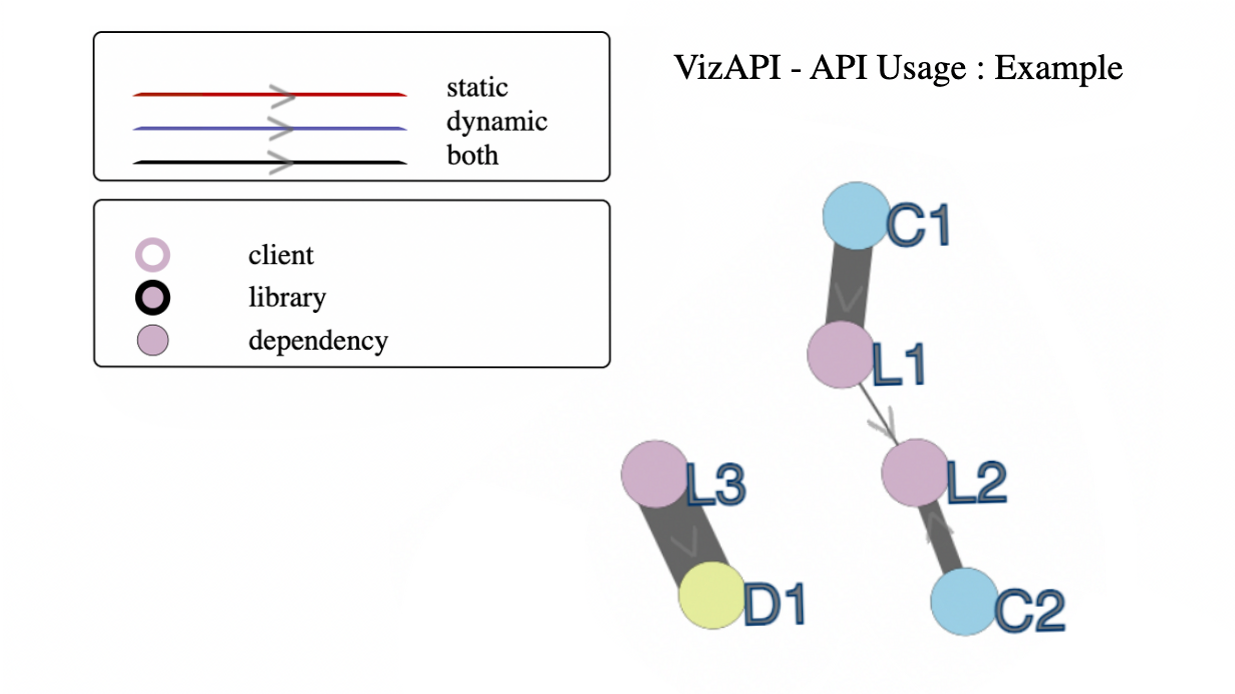
\includegraphics[height=6cm]{images/intro-example.png}
\caption{An Example VizAPI Visualization}
\label{fig:example}
\end{center}
\end{figure}

We first define the terms ``client'', ``library'' and ``dependency''. A ``client'' is a software component which directly uses some functionality of an external component, which is the ``library''. Any external component that the ``library'' directly uses is a ``dependency''. 

Figure~\ref{fig:example} illustrates a possible VizAPI usage scenario, from the perspective of a client developer. Consider a client $C$ (blue nodes) and a library $L$ (purple nodes), in the context of plain Java. Library $L$ has packages $L_1$, $L_2$, and $L_3$. $C$ calls into $L_1$ and $L_2$. Internally, within $L$, $L_1$ and $L_2$ call into each other, but not into $L_3$. The VizAPI result, with no edges from $C$ directly to $L_3$, allows a developer to conclude that breaking changes in $L_3$ will not affect $C$. Also, if only $L_3$ uses an external dependency $D$ (yellow node), then we know that $C$ will not need $D$ to be on its classpath.


We next describe the design of VizAPI, including how we
collect information and format it for the d3js visualization
library. We also present two VizAPI usage scenarios.

\subsection{Visualization System}
\label{subsec:vis-system}

\begin{figure*}[h]
\begin{center}

\subfloat[Usage Scenario 1: Library \textit{jsoup} (pink with dark borders), called by two clients, \textit{ez-vcard} (hollow with purple border) and \textit{JsoupXpath} (hollow with pink border). Exploration shows that internal jsoup packages aren't called directly by clients.
\label{fig:usagescenario1}]
{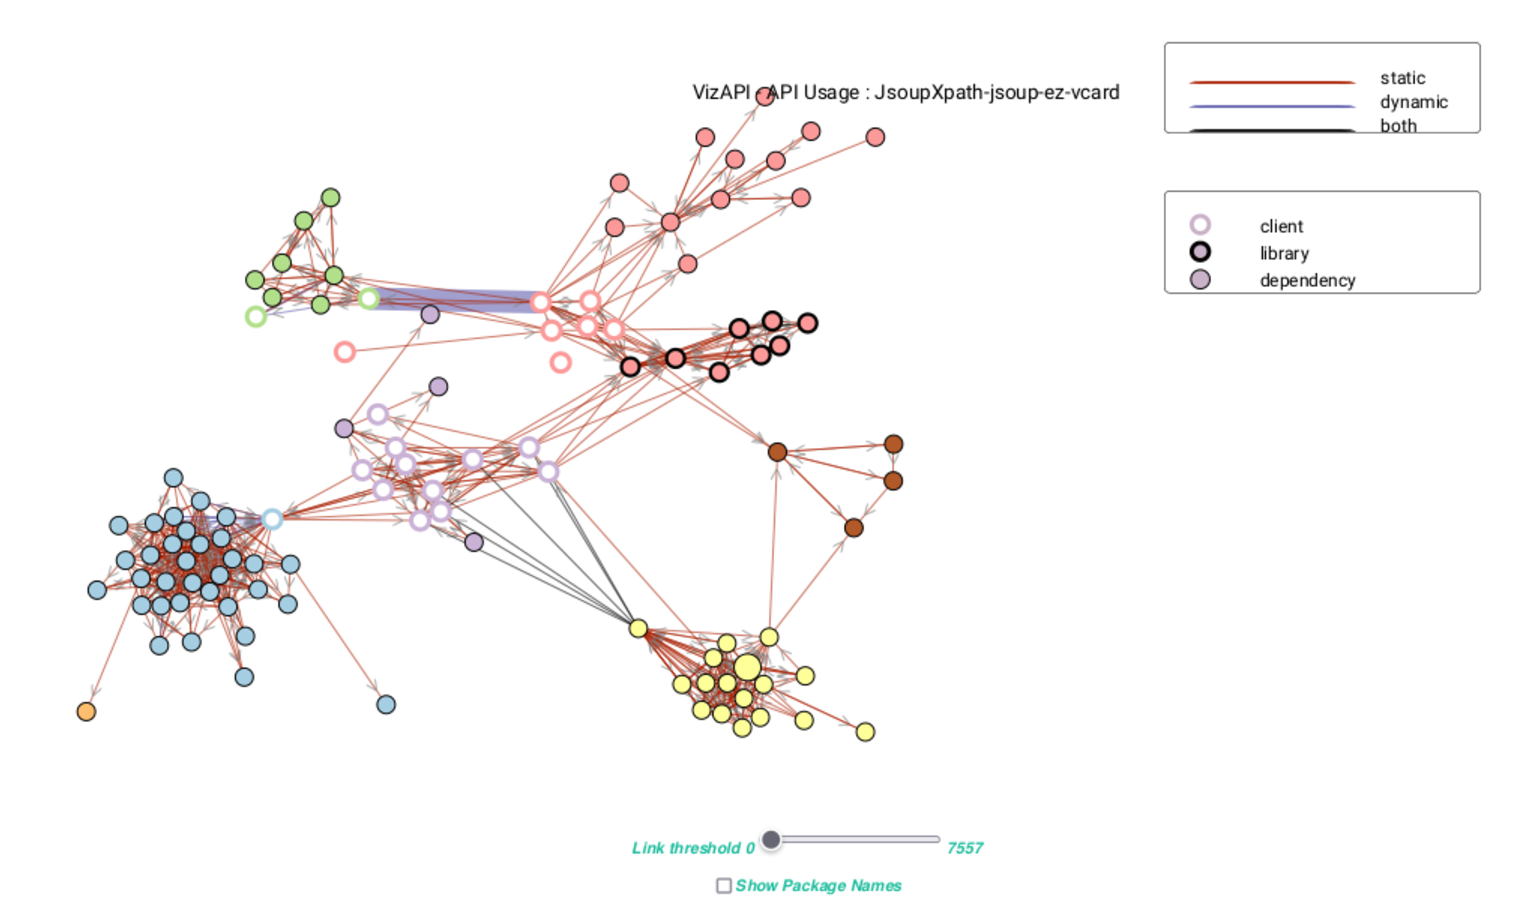
\includegraphics[width=16cm]{images/usage-scenario1.pdf}}
\hspace{7mm}

\subfloat[Usage Scenario 2: Client \textit{dataprocessor} (hollow, orange border) calls only one package in library \textit{fastjson} (green fill).
\label{fig:usagescenario2}]
{
\makebox[16cm]{
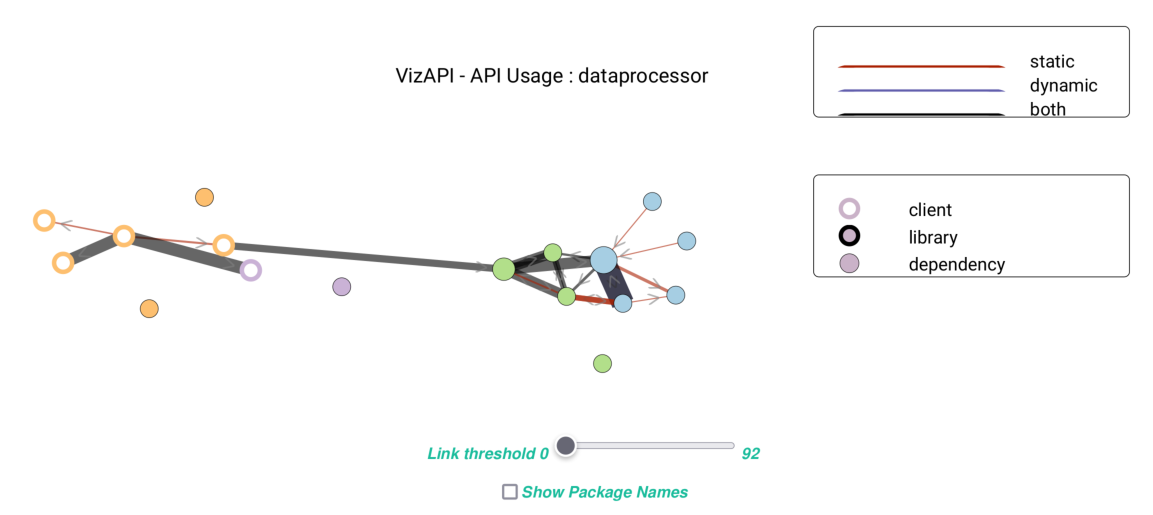
\includegraphics[width=11cm]{images/usage-scenario2.pdf}
}
}
\caption{\label{fig:usagescenarios} VizAPI Usage Scenarios.}

\end{center}
\end{figure*}


Once we have generated data from our tool that runs the static and dynamic analyses, we use a modified version
of the d3graph\footnote{\url{https://pypi.org/project/d3graph/}} library in Python to generate a d3js\footnote{\url{https://d3js.org/}}
visualization. The modifications that we made to the d3graph  library in Python in Python include multiple styling changes (for example, changing node styles based on whether it is a client, library or dependency),
legends and a toggle to show all package names. 
The graphs in Figures~\ref{fig:example}, \ref{fig:usagescenario1} and \ref{fig:usagescenario2} are examples of graphs produced by VizAPI.

VizAPI graphs are force-directed graphs based on the frequency of
interactions between different software components.  Each node is a
set of one or more packages that belong to the same JAR.  There are
three categories of nodes: clients are represented by nodes with white
interiors; libraries by nodes with filled interiors and black borders;
and dependencies (called by libraries but not clients) by nodes with
filled interiors and normal borders.  We coalesce nodes if they
originate from the same JAR and have the same incoming and
outgoing edges.

Each edge is directed
from the source package(s) to the target package(s) and represents an interaction 
(invocations, fields, annotations, subtyping) between packages. 
The thickness of each edge reflects the frequency of interactions between the source and the target.
Double-clicking on a node emphasizes its direct interactions with other packages while fading out the rest of the graph.

We run a Python implementation of the Louvain clustering algorithm~\cite{blondel2008fast}, and make the clusters 
visible by colouring nodes based on cluster.
This means that the same colour could indicate nodes (of the same category) from the same or different JARs.
Hovering on a node shows the list of packages and 
the JAR that they belong to, 
formatted as “jar : $\langle$space separated list of packages$\rangle$”. 

\subsection{Case Study}
\label{subsec:evaluation}

We conducted a pilot study of VizAPI.
We have generated data from our benchmarks.
We have collected both static and dynamic data for these projects, 
and we are in a position
to generate graphs for combinations of clients and libraries
in these projects. 
We present two usage scenarios below; graphs for 
our usage scenarios are publicly available.\footnote{\url{https://sruthivenkat.github.io/VizAPI-graph/}}
We intend for these usage scenarios to show how VizAPI can be useful to client developers when they want to observe library API usage and for library developers when they want to observe how their library is used by clients.

\paragraph{Usage Scenario 1: jsoup}
Imagine that we are a jsoup developer and want to understand
how some clients interact with it, in anticipation of making some breaking changes. We choose clients JsoupXpath\footnote{\url{https://github.com/zhegexiaohuozi/JsoupXpath}\label{jsoupxpath}} and ez-vcard\footnote{\url{https://github.com/mangstadt/ez-vcard}\label{ez-vcard}}.
Figure~\ref{fig:usagescenario1} shows static and dynamic interactions of the 2 clients with the jsoup\footnote{\url{https://github.com/jhy/jsoup}\label{jsoup}} library. Recall that nodes represent packages and edges represent interactions (usually invocations) between packages. 

We can start our exploration with the cluster of pink nodes. Many of these nodes belong to either JsoupXpath or jsoup. Hovering over a node tells us the package names while double-clicking shows us its direct interactions. (To search for a package, we can click on ``show package names'' and use the browser's find functionality.) Here, client JsoupXpath calls directly into \texttt{org.jsoup.nodes} and \texttt{org.jsoup.select}. Notably, and as we might expect, we can see that \texttt{org.jsoup.helper} and \texttt{org.jsoup.internal} aren't called directly by JsoupXpath. This would mean that breaking changes in \texttt{org.jsoup.helper} or \texttt{org.jsoup.internal} wouldn't directly affect JsoupXpath\footnote{As a specific example, the retraction of an internal jsoup API would not break this client. Behavioural changes that are directly passed through to the external API, for example, through delegation, can still break clients, but we can consider those to be changes in the external API.} 

Similarly, ez-vcard, which belongs to the purple cluster in Figure~\ref{fig:usagescenario1}, directly calls into \texttt{org.jsoup}. ez-vcard also calls into jackson-core\footnote{\url{https://github.com/FasterXML/jackson-core}\label{jackson-core}} and jackson-databind\footnote{\url{https://github.com/FasterXML/jackson-databind}\label{jackson-databind}}, which are very tightly coupled amongst their own packages and with each other. As a jsoup developer, we would be indifferent since it does not affect us; others, however, can observe that breaking changes in jackson-core and jackson-databind could propagate.

\paragraph{Usage Scenario 2: dataprocessor}

Figure~\ref{fig:usagescenario2} presents a second usage scenario. Here, say we are the developers of client dataprocessor\footnote{\url{https://github.com/dadiyang/dataprocessor}\label{dataprocessor}} (hollow with orange border). This client uses the fastjson\footnote{\url{https://github.com/alibaba/fastjson}\label{fastjson}} library (green fill). Our visualization shows calls only from dataprocessor package \texttt{com.github.dataprocessor.slice}, which is the orange-bordered client node (identity of the package available by hovering) to the package \texttt{com.alibaba.fastjson}. No other parts of dataprocessor use fastjson. This means that when we, as dataprocessor developers, need to upgrade the fastjson version, we only need to inspect the source code in our \texttt{com.github.dataprocessor.slice} package and cross-reference against release notes for fastjson. 

Note also the disconnected nodes in Figure~\ref{fig:usagescenario2}. These are all packages of fastjson that are not used by dataprocessor: any breaking changes in these packages definitely do not directly affect dataprocessor, and are less likely to affect it overall than packages that are directly used.

\section{Library Fission}
\label{sec:fission}
Modern software extensively reuses existing functionality using third-party libraries. Over time, libraries tend to extend their functionality, introducing more features and modifying existing ones. This leads to huge library sizes, a lot of which goes unused by a client that imports it. We have observed that modern API surfaces are vast and include thousands of potential access points, of which only hundreds are used by any typical client.This is called software bloating and there has been work around debloating. Debloating focuses on a single client at a time; it depends on dynamic analysis based on the client’s execution. We instead propose library fission, which focuses on splitting libraries based on client usage. This is a more permanent solution to bloating and does not require running analyses on clients for every execution. (We aim to split libraries based on client behaviour in a way that sub-modules of the fissioned library have common functionality.) 

We use the data generated by our static and dynamic analyses to experiment with fissioning a subset of our corpus of libraries. On a high level, by library fission, we mean that we separate packages of a library into different Maven submodules. The following are the steps we follow to perform library fission for a given library, $L$:
\begin{enumerate}
\item Filter out all interactions with $L$, i.e., client uses of $L$, $L$'s uses of dependencies and intra-library uses of $L$.
\item Run the Louvain clustering algorithm on the filtered data where each node is set to be a package belonging to a jar.
\item Split up $L$ into Maven submodules based on the clusters.
\item Test on a random subset of $L$'s clients.
\end{enumerate}

We now discuss specific examples from our libraries.

\subsection{\emph{fastjson}}
\label{sec:fastjson-fission}

We have 26 clients for \emph{fastjson}. Based on the usages of these clients, we obtained the following initial set of 5 clusters:
\begin{itemize}
\item Cluster 1:
\begin{itemize}
\item \texttt{com.alibaba.fastjson.annotation}
\item \texttt{com.alibaba.fastjson.asm}
\item \texttt{com.alibaba.fastjson.parser}
\item \texttt{com.alibaba.fastjson.serializer}
\item \texttt{com.alibaba.fastjson.support.hsf}
\item \texttt{com.alibaba.fastjson.support.config}
\item \texttt{com.alibaba.fastjson.support.retrofit}
\item \texttt{com.alibaba.fastjson.support.springfox}
\end{itemize}
\item Cluster 2:
\begin{itemize}
\item \texttt{com.alibaba.fastjson}
\end{itemize}
\item Cluster 3:
\begin{itemize}
\item \texttt{com.alibaba.fastjson.util}
\item \texttt{com.alibaba.fastjson.parser.deserializer}
\end{itemize}
\item Cluster 4:
\begin{itemize}
\item \texttt{com.alibaba.fastjson.support.spring}
\item \texttt{com.alibaba.fastjson.support.spring.annotation}
\end{itemize}
\item Cluster 5:
\begin{itemize}
\item \texttt{com.alibaba.fastjson.support.jaxrs}
\end{itemize}
\end{itemize}

We observe that the clusters are loosely based on functionality, that is, the packages within a cluster have similar functionality. This is not strictly true for all packages, but it is a good approximation. We see that the \texttt{jaxrs} and \texttt{spring} functionalities are clusters of their own and it makes sense to separate these into submodules since they provide their own independent functionality. However, we observed that there exist cyclic dependencies between Cluster 1, 2 and 3. If a library developer performs library fission and they run into cyclic dependencies, we recommend that they resolve these dependencies by moving classes into appropriate submodules. Due to our lack of domain knowledge (we don't know about what individual \emph{fastjson} classes do), we combined these 3 clusters into one submodule. Our final submodules are as follows:
\begin{itemize}
\item Submodule 1 --- utils:
\begin{itemize}
\item \texttt{com.alibaba.fastjson.annotation}
\item \texttt{com.alibaba.fastjson.asm}
\item \texttt{com.alibaba.fastjson.parser}
\item \texttt{com.alibaba.fastjson.serializer}
\item \texttt{com.alibaba.fastjson.support.hsf}
\item \texttt{com.alibaba.fastjson.support.config}
\item \texttt{com.alibaba.fastjson.support.retrofit}
\item \texttt{com.alibaba.fastjson.support.springfox}
\item \texttt{com.alibaba.fastjson}
\item \texttt{com.alibaba.fastjson.util}
\item \texttt{com.alibaba.fastjson.parser.deserializer}
\end{itemize}
\item Submodule 2 --- spring:
\begin{itemize}
\item \texttt{com.alibaba.fastjson.support.spring}
\item \texttt{com.alibaba.fastjson.support.spring.annotation}
\end{itemize}
\item Submodule 3 --- jaxrs:
\begin{itemize}
\item \texttt{com.alibaba.fastjson.support.jaxrs}
\end{itemize}
\end{itemize}

When we split \emph{fastjson} into submodules, we observed that each submodule needed fewer dependencies in the pom compared to the current version of \emph{fastjson} that is not split. The current version of \emph{fastjson} has 61 dependencies, while \emph{utils} has 47, \emph{spring} has 27 and \emph{jaxrs} has 29. Importing one of these newer submodules means a smaller probability of propagated vulnerabilities, version conflicts and breaking changes.

We sent an email to the \emph{fastjson} contributors proposing a split and did not receive a response, after which we created a pull request\footnote{\url{}https://github.com/alibaba/fastjson/pull/4276}. Our PR text was as follows:
``This PR splits fastjson into 3 submodules - utils, spring, jaxrs. We're looking into Java API usage as part of research and propose this split. These submodules are based on usage patterns that we've observed clients making of fastjson. It is beneficial to clients – they can import only the submodule they need to use (utils seems to be most popular). After this change, clients will not be affected by breaking changes in unused submodules and can avoid version conflicts and vulnerabilities propagated through dependencies. We believe that this split makes it easier to release backward compatible versions of fastjson and to isolate breaking changes."

We looked for \emph{fastjson}'s vulnerabilites using the ``Synk Vulnerability DB" and found the ``Unsafe deserialization in com.alibaba:fastjson" vulnerability which affects versions < 1.2.83. Following this, we inspected the source code for the fix and found that the vulnerability originates in the \emph{utils} cluster. Using Github's advanced search, we went through 10 projects that use \emph{fastjson} and found that while 6 of them use \emph{utils} and will continue to be vulnerable, the vulnerability will not be reported for 4 of the projects after fission.

\subsection{\emph{jsoup}}
\label{sec:jsoup-fission}

Based on usage by the 7 clients of jsoup we have in our benchmark set, we observed the following clusters:
\begin{itemize}
\item Cluster 1:
\begin{itemize}
\item \texttt{org.jsoup.parser}
\item \texttt{org.jsoup.safety}
\item \texttt{org.jsoup.helper}
\item \texttt{org.jsoup.internal}
\end{itemize}
\item Cluster 2:
\begin{itemize}
\item \texttt{org.jsoup}
\item \texttt{org.jsoup.examples}
\end{itemize}
\item Cluster 3:
\begin{itemize}
\item \texttt{org.jsoup.select}
\item \texttt{org.jsoup.nodes}
\end{itemize}
\end{itemize}

We observed multiple cyclic dependencies. In the case of cyclic dependencies, it is best for the library developers to split classes in packages and move them to clusters based on functionality. 

We now discuss a few interesting things we noted in the \emph{jsoup} clusters. Cluster 1 contains \texttt{org.jsoup.internal}. It is clear from the naming that this package is meant for internal use only and not for clients. We suggest that such packages be moved to a separate submodule so that clients are not tempted to import them. Similarly, Cluster 2 contains \texttt{org.jsoup.examples} which also almost certainly will not be needed by clients and can also be moved to a separate submodule. 

Due to the multiple cyclic dependencies that we observed, we did not raise a pull request for \emph{jsoup}.

\subsection{\emph{guava}}
\label{sec:guava-fission}

The \emph{guava} library makes an interesting case for library fission since it provides multiple functionalities such as I/O, caching, collections and so on, all within the same library. Due to this, we see multiple clusters for the library as expected. In this library too, we observe that packages have loosely similar functionality within clusters. Our final submodules for \emph{guava} are as follows:

\begin{itemize}
\item Submodule 1 --- annotations:
\begin{itemize}
\item \texttt{com.google.common.annotations}
\end{itemize}
\item Submodule 2 --- eventbus:
\begin{itemize}
\item \texttt{com.google.common.eventbus}
\end{itemize}
\item Submodule 3 --- reflect:
\begin{itemize}
\item \texttt{com.google.common.reflect}
\end{itemize}
\item Submodule 4 --- html-xml:
\begin{itemize}
\item \texttt{com.google.common.html}
\item \texttt{com.google.common.xml}
\end{itemize}
\item Submodule 5
\begin{itemize}
\item \texttt{com.google.common.escape}
\item \texttt{com.google.common.io}
\item \texttt{com.google.common.net}
\item \texttt{com.google.common.graph}
\end{itemize}
\item Submodule 6
\begin{itemize}
\item \texttt{com.google.common.base}
\item \texttt{com.google.common.cache}
\item \texttt{com.google.common.collect}
\item \texttt{com.google.common.hash}
\item \texttt{com.google.common.math}
\item \texttt{com.google.common.primitives}
\item \texttt{com.google.common.util}
\end{itemize}
\end{itemize}

We looked at the ``Synk Vulnerability DB" for \emph{guava}. We found two vulnerabilties, ``Information Disclosure" which affects the ``com.google.common.io" package and ``Deserialization of Untrusted Data" which affects the ``com.google.common.collect" package. When we combed through projects that depend on \emph{guava} using Github's advanced search, we found multiple projects that depend on the invulnerable packages of \emph{guava} and would potentially benefit from fissioning \emph{guava}, in terms of security vulnerabilities.

We believe that library fission is potentially beneficial to developers. However, we expect developer resistance when it comes to making these changes in their libraries since they are breaking changes. Tran et al ~\cite{tran2000architectural} look into repairing 2 open source systems (Linux and VIM) and Dr. Michael W. Godfrey explained to us that while the developers of these systems were appreciative of the changes they had made, they were still reluctant to accept them due to the fact that they were breaking changes (personal communication, September 21, 2022). We believe that the appropriate window to introduce fission changes is when other major breaking changes are being planned. The main breaking change that library fission introduces in a client is that the client needs to identify the submodules that it requires and import only those submodules. We expect no impacts on clients in terms of performance since we are only adding visibility limitations. The worst case that we foresee is that a client requires all the submodules of the library, in which case there is no difference from the previous version of the library that was not fissioned. We tested library fission on a subset of libraries and a random subset of their clients from our benchmarks--the unit test results were the same and we observed no change in build times.



\section{Upgrades, Breaking Changes and Backward Compatibility}
Our data for 101 Java software components contains different kind of interactions across component boundaries. This data can be analyzed and prove useful in the following ways:
\begin{itemize}
\item Library developers can observe different usage patterns of their APIs. The clusters observed in library packages can help with new version releases. Breaking changes might be restricted to clusters and library developers can choose whether to make clusters from new versions backward compatible with other clusters from older versions or not. 
\item Clients can also check if breaking changes in new library versions will affect their code during upgrades and cross check this with library changelogs. 
\item Unused dependencies can be identified and removed to prevent them from possibly introducing version conflicts and vulnerabilties.
\end{itemize}